\documentclass[11pt,a4paper]{article}
\usepackage[margin=2.2cm]{geometry}
\usepackage{graphicx,booktabs,amsmath,xcolor}
\usepackage[hidelinks]{hyperref}
\usepackage[font=small,labelfont=bf]{caption}
\newcommand{\pc}{p_c}
\title{Overnight simulations: adaptive methods, trial numbers and a shorter experiment}
\author{av-dur v2 \quad 28 October 2026}
\date{}
\begin{document}
\maketitle
\vspace{-1.5em}

\section*{Summary}
\begin{enumerate}
\item \textbf{Main (bimodal) experiment: 9 conflicts ($\pm$450\,ms) at about 70 trials per condition, with $\sigma_V$ taken from the unimodal visual block.} The current design (7 conflicts, $\pm$250\,ms, 154 trials, 111\,min) recovers the right model for only 48\% of simulated participants. Causal inference is recognised in 42\% of cases, and more trials do not help the 7-conflict design (47\% at 90 trials per condition). With 9 conflicts and 60 trials per condition (56\,min), the right model is recovered for 72\% (AIC). Fixing $\sigma_V$ from the unimodal block raises this to 83\%, and $p_c$ is then recovered with an RMSE of 0.17 instead of 0.34. More trials help less than either change.
\item \textbf{Unimodal blocks: keep QUEST+ (PSE and slope).} At 100 trials it measures $\sigma$ with a log error of about 0.21. The old four staircases do not reach that even at 200 trials. Because $\sigma_V$ now matters for the main fit, I suggest 100 visual trials instead of 70 (+1.5\,min).
\item \textbf{Cross-modal block: the method matters little; the number of participants matters most.} QUEST+ targeting only the PSE is the best method, as your friend said, but it saves only 0--25\% of the trials compared with the current staircases. The bias growth term $d$ differs more between participants (SD about 0.26--0.30) than it is measured within one participant (SE 0.08--0.18). A short 3-standard design for everyone is therefore better than a long one for 6 participants.
\item \textbf{Main experiment: keep the staircases, not QUEST+} (added 28 Oct, midday). At 72 trials per condition, with $\sigma_V$ shared as in your joint fit, the current staircases recover the right model for 90\% of simulated participants. QUEST+ targeting PSE and slope reaches 86\%, and QUEST+ targeting the PSE only also 86\%. The paired difference is $-4$ points (95\% CI $-9$ to $+1.5$), and $p_c$ comes out equally well with every method (RMSE 0.16--0.18). QUEST+ targeting PSE and slope measures each condition's PSE worse (61 vs 47\,ms at low noise). QUEST+ neither shortens the main experiment nor makes it more precise (Section~\ref{sec:qplus}).
\item \textbf{Together:} the session goes from about 176 to about 126 minutes, and every participant gets all three cross-modal standards (Table~\ref{tab:plan}).
\end{enumerate}

\begin{table}[h]
\centering\small
\begin{tabular}{lrrrr}
\toprule
 & \multicolumn{2}{c}{current} & \multicolumn{2}{c}{proposed} \\
\cmidrule(lr){2-3}\cmidrule(lr){4-5}
block & trials & min & trials & min \\
\midrule
noise calibration (not simulated) & 206 & 11 & 206 & 11 \\
practice & 20 & 1 & 20 & 1 \\
unimodal auditory, QUEST+ (2 noise $\times$ (90 + 14 easy)) & 208 & 11 & 208 & 11 \\
unimodal visual, QUEST+ (70\,$\to$\,100 + 14 easy) & 84 & 4 & 114 & 6 \\
cross-modal, 3 standards (now 6 people; then all, 3 $\times$ 100 per noise) & 732 & 38 & 600 & 31 \\
main, 2 noise $\times$ 7 conflicts $\times$ 154 $\to$ 9 conflicts $\times$ 72 & 2156 & 111 & 1296 & 67 \\
\midrule
total & 3406 & 176 & 2444 & 126 \\
\bottomrule
\end{tabular}
\caption{Session length at the measured 3.1\,s per trial, including cues and breaks (P102's interleaved cross-modal session: 732 trials in 37.7\,min). The current cross-modal row is the 6-participant subset; for everyone else it is 388 trials (20\,min).}
\label{tab:plan}
\end{table}

\section{What was simulated}
\paragraph{Adaptive blocks} (\texttt{adaptive\_sims.py}). Each simulated run is 200 trials of one condition, 7\% of them easy trials, scored after its first 40--200 trials with the experiment's lognormal fit (lapse 0--0.1). There were 500 observers per task, plus 250 per robustness variant.
\begin{itemize}
\item Observers: auditory at low noise ($\sigma \sim U(0.12, 0.45)$), auditory at high noise ($U(0.5, 1.1)$) and visual ($U(0.3, 1.0)$). Cross-modal observers have a bias: PSE ln-ratio $U(-0.6, -0.05)$ at low noise and $U(-0.6, 0.05)$ at high noise.
\item Robustness variants: lapse 0.15; learning ($\sigma$ falls by 40\% and the PSE drifts by 0.1 over the run); order bias 0.15.
\item Methods:
  \begin{itemize}
  \item QUEST+ targeting the PSE and slope (the current unimodal design).
  \item QUEST+ targeting the PSE only.
  \item The old unimodal staircases: 2D1U and 3D1U from the floor, 1D2U and 1D3U from the ceiling.
  \item The current cross-modal staircases: two 1D1U, plus 2D1U and 1D2U.
  \item Two 1D1U only (the 300/800\,ms design).
  \end{itemize}
\end{itemize}

\paragraph{Main experiment} (\texttt{bimodal\_recovery.py}).
\begin{itemize}
\item Simulated participants follow causal inference (CI), forced fusion or switching (163 participants, 54--55 per model). The models are those of \texttt{monteCarloClass}, with the likelihood computed exactly by quadrature.
\item Parameters: $\lambda \sim U(0.001, 0.1)$; $\sigma_{A,\text{low}} \sim U(0.12, 0.45)$; $\sigma_{A,\text{high}} \sim U(0.55, 1)$; $\sigma_V \sim U(0.3, 1)$; $p_c$ and $p_\text{switch} \sim U(0.1, 0.9)$.
\item Every condition (noise $\times$ conflict) runs exactly as in the experiment: a 2D1U staircase from the floor and a 1D2U from the ceiling (floor $-95\%$, ceiling $+90\%$), easy trials, and whole frames at 120\,Hz.
\item Shorter designs use the first $n$ trials of the same run, as if the session had stopped early.
\item Each data set was fitted with all three models by BADS (3 starts each). CI was also started from the fusion solution, so it can never fit worse than fusion (it did not in any case).
\item \texttt{fixed\_sv.py} refitted the same participants' data with $\sigma_V$ fixed at the true value $\times\, e^{N(0, 0.25)}$, i.e.\ with the error of a 70-trial unimodal visual QUEST+ block. This covered 140 participants (46 per model) and 3 designs.
\item No audiovisual bias was simulated. The results therefore assume the bias is modelled well (Section~\ref{sec:ideas}).
\end{itemize}

\section{Unimodal blocks}
\begin{figure}[h]
\centering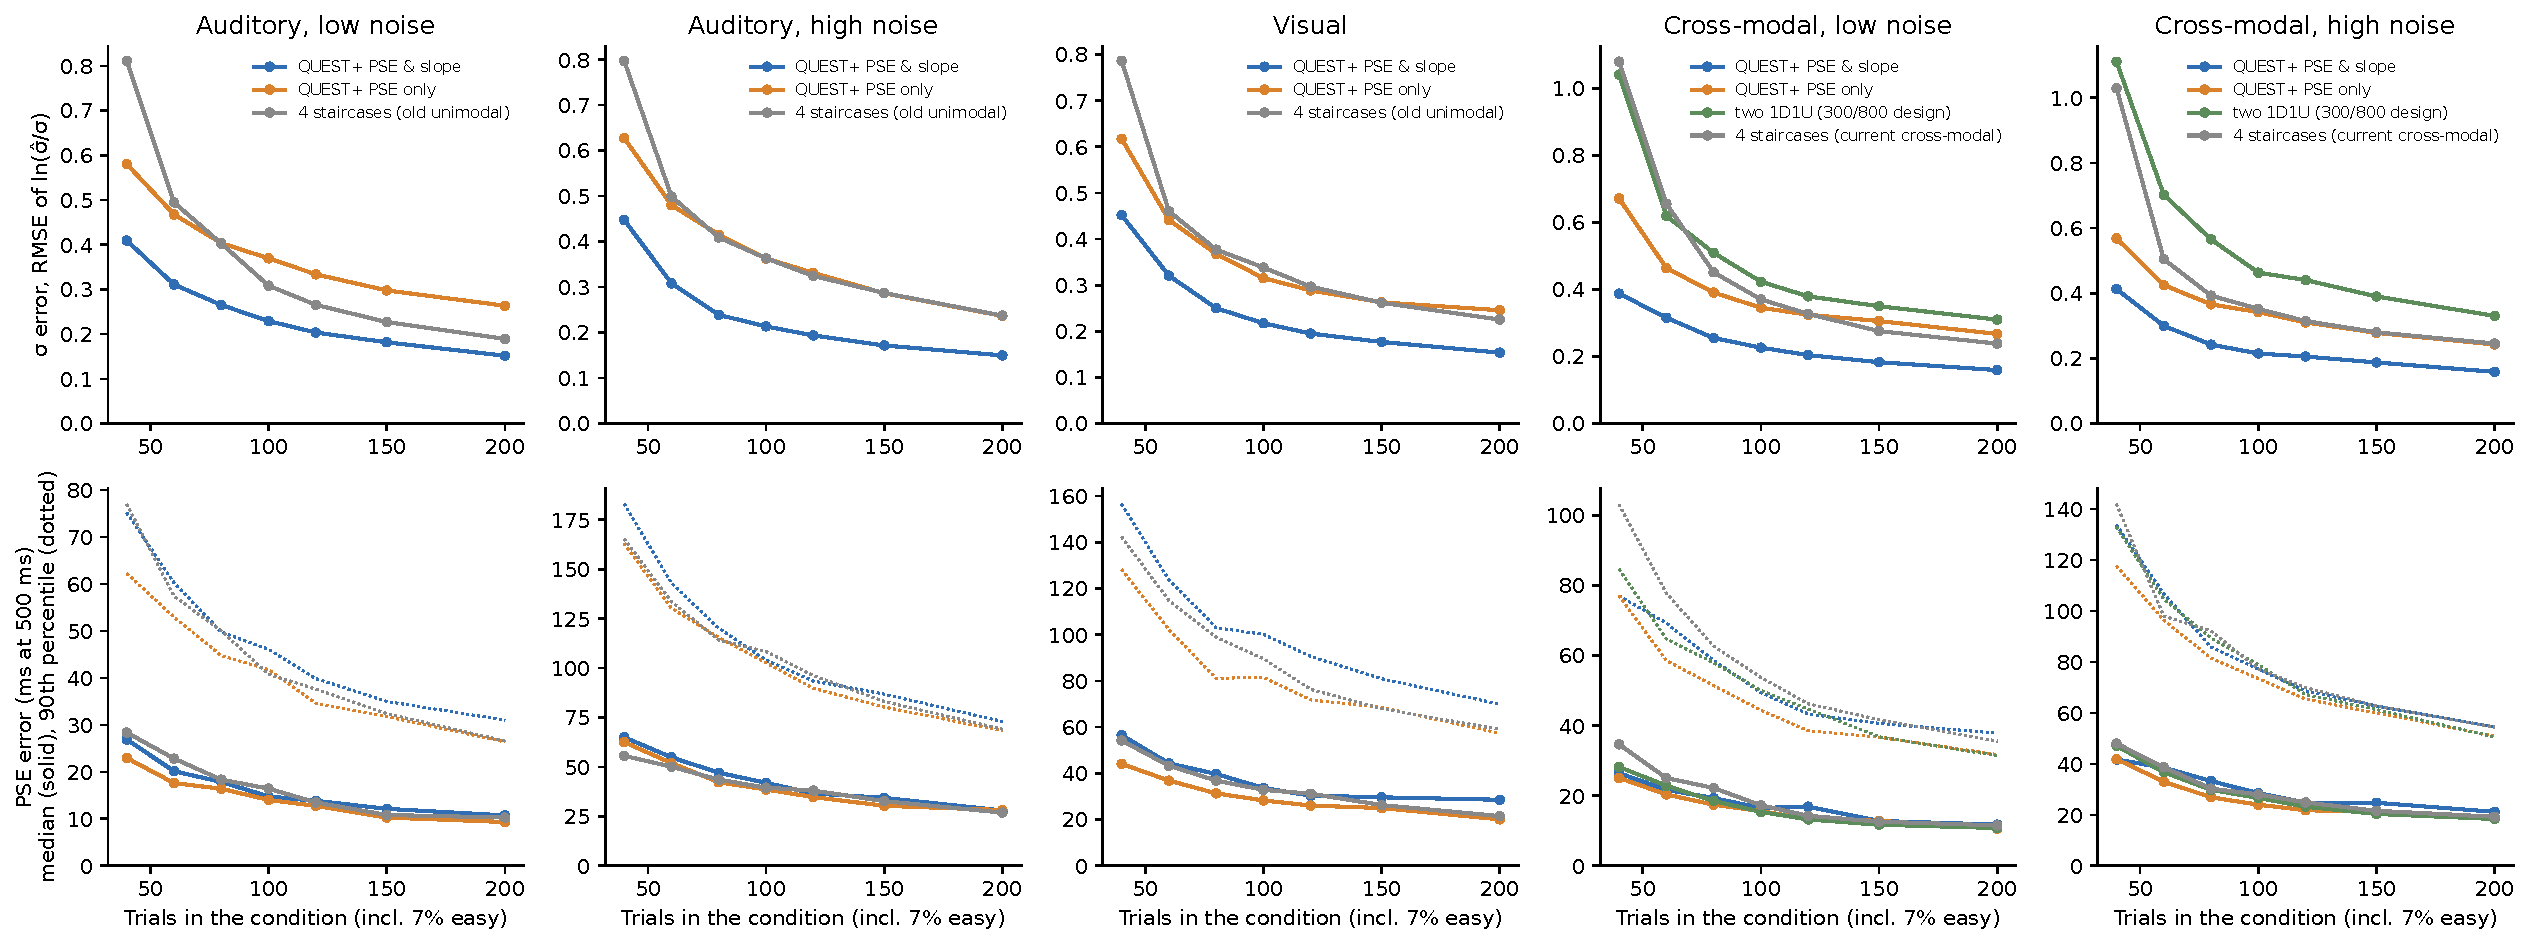
\includegraphics[width=\linewidth]{fig_adaptive.pdf}
\caption{Top: error of the slope $\sigma$ (RMSE of $\ln\hat\sigma/\sigma$). Bottom: PSE error in ms at 500\,ms (median solid, 90th percentile dotted). Horizontal axis: trials in the condition.}
\label{fig:adaptive}
\end{figure}

QUEST+ with PSE and slope gives the best $\sigma$ by far (Fig.~\ref{fig:adaptive}, top). At 100 trials the error is 0.21--0.23 in every task. The old staircase design reaches the same error only at about 150 trials at low noise, and not within 200 trials at high noise or for vision.

For the PSE, all methods are within about 15\% of each other (bottom row). QUEST+ with PSE and slope occasionally fails at high auditory noise (PSE error above 150\,ms in 3.8\% of runs at 100 trials, against 2.2\% for the staircases). That does not matter here, because the unimodal block is there for $\sigma$.

QUEST+ targeting the PSE only underestimates $\sigma$ (bias $-0.10$ to $-0.13$ in log units at 100 trials), because it places almost all of its trials at the PSE.

\paragraph{Recommendation.}
\begin{itemize}
\item Keep the current QUEST+ blocks.
\item Auditory: 90 trials per noise level puts $\sigma$ at about 0.22; more trials buy little (0.17 at 150).
\item Visual: 70 trials puts $\sigma_V$ at about 0.26. Since the main fit now leans on $\sigma_V$ (Section~\ref{sec:bimodal}), 100 trials (error 0.22) is worth the extra 1.5 minutes.
\end{itemize}

\section{Cross-modal block}
\paragraph{Method.} QUEST+ targeting the PSE only is the best method for the PSE, but only by a little. To match its precision at 100 trials, the current four staircases need 112 trials at low noise and 132 at high noise, and two 1D1U need 99 and 120. Under the robustness variants (lapse 0.15, learning, order bias) it was never worse than the staircases. With a lapse of 0.15 it matched two 1D1U and beat the current four staircases (median error 13 vs 15\,ms at 200 trials).

The PSE-only QUEST+ gives a poor $\sigma$, but the cross-modal $\sigma$ is not needed, because $\sigma_A$ and $\sigma_V$ come from the unimodal blocks. Switching to it is reasonable, but it is not where the time savings are.

\paragraph{Allocation over the three standards.} For each participant, $c$ and $d$ were fitted from the simulated PSEs at 300/500/800\,ms. The standard error of $d$, low / high noise, under each allocation:

\begin{center}\small
\begin{tabular}{lcccc}
\toprule
trials per standard & total & min & SE($d$), staircases & SE($d$), QUEST+ PSE \\
\midrule
86/194/86 (current) & 732 & 38 & 0.12 / 0.17 & 0.10 / 0.14 \\
122/122/122 & 732 & 38 & 0.09 / 0.14 & 0.08 / 0.13 \\
60/120/60 & 480 & 25 & 0.15 / 0.20 & 0.13 / 0.18 \\
100/100/100 & 600 & 31 & \multicolumn{2}{c}{about 0.09--0.15 (interpolated)} \\
\bottomrule
\end{tabular}
\end{center}

Splitting the trials equally improves $d$ at no cost in time. It costs a little precision in $c$ at 500\,ms (SE 0.056 vs 0.044), which the shared model makes up for.

\paragraph{How many participants.} Between participants, $d$ varies a lot: P101, P102 and P104 give an SD of 0.26 (low noise) and 0.30 (high noise). That is about twice each participant's measurement error. The standard error of the group mean $d$ is $\sqrt{(\text{SD}^2 + \text{SE}^2)/N}$:
\begin{center}\small
\begin{tabular}{lcccc}
\toprule
& $N = 3$ & 6 & 12 & 20 \\
\midrule
SE of the group $d$ (SD 0.26--0.30, SE 0.08--0.18) & 0.16--0.20 & 0.11--0.14 & 0.08--0.10 & 0.06--0.08 \\
\bottomrule
\end{tabular}
\end{center}
Cutting a participant's trials from 732 to 480 raises the group SE by less than 10\%, whereas going from 6 to 12 participants lowers it by 30\%.

Two more reasons favour everyone. $d$ evidently differs between participants (P104 shows the opposite sign at low noise), so a model with $d$ per participant needs every participant to have all three standards. And a self-selected subset of 6 leaves the other participants' bias at 50 or 950\,ms purely extrapolated.

\textbf{Recommendation:} all three standards for everyone (\texttt{n\_participants=None}), 100 trials per standard and noise level, 31\,min.

\section{Main experiment}\label{sec:bimodal}
\begin{figure}[h]
\centering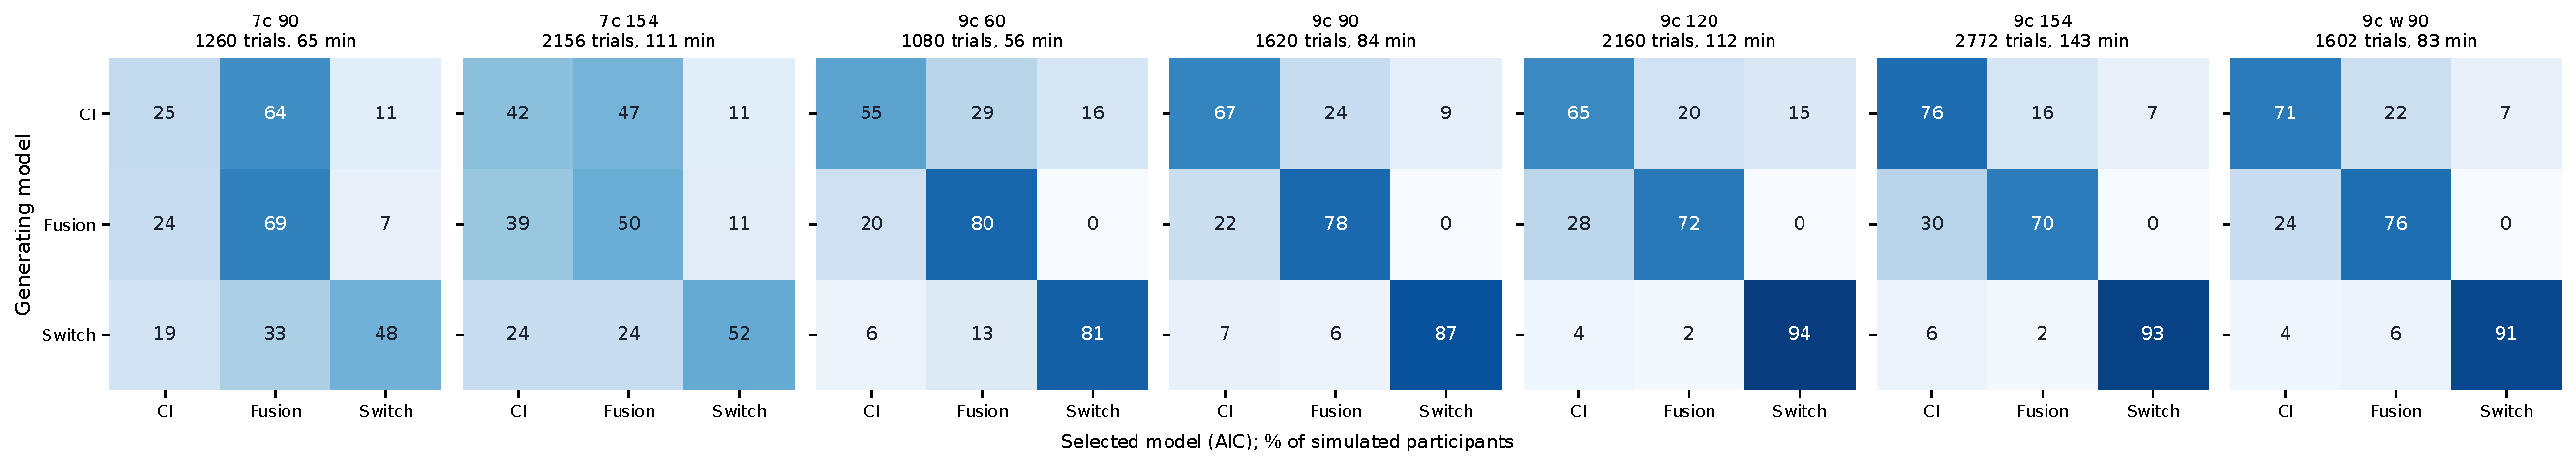
\includegraphics[width=\linewidth]{fig_confusion.pdf}
\caption{Model recovery by AIC: rows are the generating model, columns the selected model (\% of 54--55 simulated participants per model). Above each panel: trials and minutes for the main experiment.}
\label{fig:conf}
\end{figure}

\paragraph{9 vs 7 conflicts.} With conflicts up to $\pm$250\,ms, the three models make almost the same predictions (Fig.~\ref{fig:conf}). Even at 154 trials per condition, 7 conflicts identify CI in only 42\% of cases (25\% at 90), and CI is mostly mistaken for fusion. 9 conflicts up to $\pm$450\,ms do better in half the time: at 60 trials per condition (56\,min) the mean recovery is 72\%, against 48\% for the current 111-minute design.

The large conflicts are where CI breaks away from fusion, and the extra range helps far more than extra trials do. Beyond 90 trials per condition recovery barely improves: 77\% at 90 and 120 trials, 80\% at 154 (Fig.~\ref{fig:time} in the appendix).

\textbf{Moving trials to the large conflicts} (0 and $\pm$112\,ms $\times$0.7, $\pm$338 and $\pm$450\,ms $\times$1.2) made no difference: 79\% vs 77\%, within the simulation error of about $\pm$6 points. It is not worth the added complexity.

\paragraph{AIC vs BIC.} BIC penalises CI's extra parameter heavily. It picks fusion for almost every fusion participant, but for only 31--51\% of CI participants (2\% with 7 conflicts). If model comparison is reported per participant, AIC (or cross-validation) is the fairer criterion.

\paragraph{Parameters.} $\sigma_A$ is recovered well in every design (log RMSE 0.10--0.16 at low noise, 0.15--0.23 at high noise). $\sigma_V$ is not (log RMSE 0.7--1.1): in the bimodal data, $\sigma_V$ trades off against $p_c$, since both control how far the PSE follows the visual standard. $p_c$ itself is recovered poorly when $\sigma_V$ is free (RMSE 0.29--0.37 with 9 conflicts, 0.46--0.48 with 7; Fig.~\ref{fig:ci} in the appendix).

\begin{figure}[h]
\centering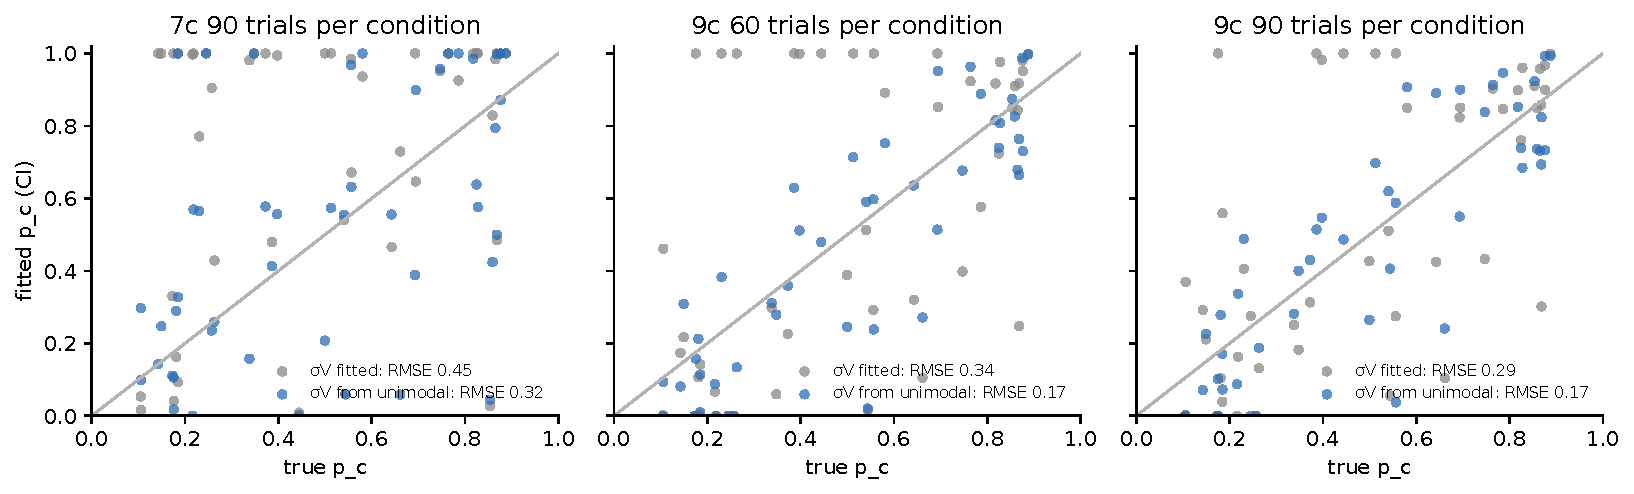
\includegraphics[width=\linewidth]{fig_fixed_sv.pdf}
\caption{Fitted vs true $p_c$ for CI participants, with $\sigma_V$ fitted (grey) or fixed from a simulated unimodal visual block (blue; log error 0.25). The same participants and the same answers are used in both cases.}
\label{fig:fixed}
\end{figure}

\paragraph{$\sigma_V$ from the unimodal block.} Fixing $\sigma_V$ at the value from the unimodal visual block, with realistic error, removes this trade-off (Fig.~\ref{fig:fixed}):
\begin{center}\small
\begin{tabular}{llcccccc}
\toprule
design & $\sigma_V$ & \multicolumn{4}{c}{correct model, AIC (BIC)} & $p_c$ RMSE & $r(p_c)$ \\
\cmidrule(lr){3-6}
 & & CI & fusion & switch & mean & & \\
\midrule
7c, 90 & fitted & 21 (0) & 68 (100) & 48 (15) & 46 (38) & 0.45 & 0.28 \\
7c, 90 & unimodal & 57 (43) & 74 (85) & 48 (17) & 60 (48) & 0.32 & 0.50 \\
9c, 60 & fitted & 57 (32) & 83 (98) & 83 (39) & 74 (56) & 0.34 & 0.55 \\
9c, 60 & unimodal & \textbf{87 (89)} & 79 (94) & 83 (46) & \textbf{83 (76)} & \textbf{0.17} & \textbf{0.87} \\
9c, 90 & fitted & 70 (38) & 83 (98) & 89 (56) & 81 (64) & 0.29 & 0.64 \\
9c, 90 & unimodal & 89 (87) & 77 (94) & 87 (63) & 84 (81) & 0.17 & 0.86 \\
\bottomrule
\end{tabular}
\end{center}
(46 participants per model. Percentages carry a simulation error of about $\pm$6 points.)

With $\sigma_V$ fixed, 9 conflicts at 60 trials per condition recover CI in 87\% of cases, and $p_c$ correlates 0.87 with its true value. That is better than any design with $\sigma_V$ free, including 154 trials per condition. Going to 90 trials adds nothing to model recovery once $\sigma_V$ is fixed.

The remaining weak point is switching vs CI at low $p_c$: when $p_c$ is small, CI predicts auditory-only answers, much as switching with a low $p_\text{switch}$ does. More trials (and BIC) do not solve this.

This assumes that $\sigma_V$ is the same in the unimodal and bimodal tasks. A milder version is to use the unimodal $\sigma_V$ as a prior (log SD 0.25) instead of fixing it, and to test that assumption with a likelihood-ratio test against the free fit.

\paragraph{PSE per condition} (Fig.~\ref{fig:pse} in the appendix). The PSE error at 90 trials is 42\,ms at low noise and 74\,ms at high noise (RMSE over all conditions; at 154 trials, 34 and 57\,ms). It grows towards $\pm$450\,ms. That is enough for the model fit, which pools all conditions, but too noisy to read the PSE-vs-conflict curve condition by condition at high noise.

\paragraph{The extreme conflicts.} At $-450$\,ms the visual standard lasts 50\,ms. That is above the shortest flash allowed (25\,ms) but far below the cross-modal standards (300--800\,ms), so the audiovisual bias there is an extrapolation. At $+450$\,ms the visual standard (950\,ms) sits at the top of the prior range and at the test ceiling ($+90\%$ = 950\,ms). The simulations include these limits, and the staircases still converge. Section~\ref{sec:ideas} suggests cross-modal standards that cover the main experiment's visual range.

\paragraph{Recommendation.} 9 conflicts from $-450$ to $+450$\,ms at 72 trials per condition (64 staircase trials, 32 per staircase, plus 8 easy): 1296 trials, 67\,min. Use $\sigma_V$ from the unimodal block (as in your joint fit, with one $\sigma_V$ for all tasks) and AIC for model selection. The margin over 60 trials covers what the simulation leaves out: the bias model, attention lapses that change over the session, and excluded trials.

\section{QUEST+ in the main experiment}\label{sec:qplus}
\texttt{qplus\_main.py} simulates 206 participants (68--69 per generating model), the same as in the runs above. It uses 9 conflicts $\times$ 2 noise levels $\times$ 72 trials per condition (64 adaptive + 8 easy). Every participant ran the whole experiment three times, with fresh answers each time, using one of these in every condition:
\begin{itemize}
\item the current staircases: 2D1U from the floor and 1D2U from the ceiling, 32 trials each;
\item QUEST+ targeting PSE and slope (lapse as a nuisance parameter), as in the unimodal blocks;
\item QUEST+ targeting the PSE only.
\end{itemize}
QUEST+ chooses among whole-frame test durations from 25 to 950\,ms. Its prior is flat over PSE ln-ratios from $-2.5$ to 1 (at $-450$\,ms the PSE can be near $\ln 0.3$), $\sigma$ from 0.05 to 2.5, and lapse from 0 to 0.1. The easy trials also update QUEST+.

The fits stand in for your joint fit. $\sigma_V$ is fixed at its true value $\times\, e^{N(0, 0.2)}$, representing the precision of one $\sigma_V$ shared with the unimodal and cross-modal blocks. $\sigma_A$, the lapse and each model's own parameters are free.

\begin{center}\footnotesize\setlength{\tabcolsep}{3.5pt}
\begin{tabular}{lccccccccc}
\toprule
& \multicolumn{4}{c}{correct model, AIC (BIC), \%} & & & & \multicolumn{2}{c}{PSE RMSE (ms)} \\
\cmidrule(lr){2-5}\cmidrule(lr){9-10}
method & CI & fusion & switch & mean & $p_c$ RMSE & $r(p_c)$ & $\sigma_A$ ln RMSE & low & high \\
\midrule
staircases & 90 (89) & 94 (99) & 87 (53) & \textbf{90} (80) & 0.16 & 0.83 & 0.14 / 0.18 & 47 & 81 \\
QUEST+ PSE \& slope & 84 (86) & 85 (100) & 90 (69) & 86 (85) & 0.16 & 0.87 & 0.12 / 0.16 & 61 & 103 \\
QUEST+ PSE only & 90 (87) & 82 (97) & 87 (63) & 86 (82) & 0.18 & 0.85 & 0.15 / 0.17 & 47 & 79 \\
\bottomrule
\end{tabular}
\end{center}
$\sigma_A$ is given for CI and fusion participants (low / high noise). Under switching, $\sigma_A$ is poorly identified when the participant mostly reports vision (log RMSE 0.5--0.8 with every method). Paired differences from the staircases, bootstrapped over participants:
\begin{itemize}
\item model recovery (AIC): $-3.9$ points for both QUEST+ variants (95\% CI $-9.2$ to $+1.5$);
\item $p_c$ RMSE: $0.00$ ($-0.04$ to $+0.04$) for PSE and slope, and $+0.01$ ($-0.04$ to $+0.07$) for the PSE only.
\end{itemize}

\begin{figure}[h]
\centering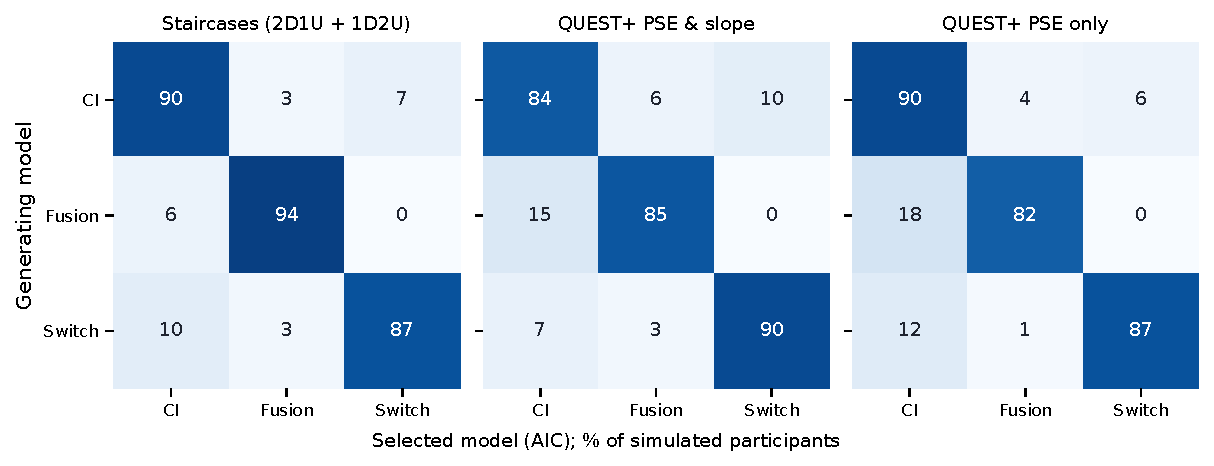
\includegraphics[width=0.75\linewidth]{fig_qplus_confusion.pdf}\\[2pt]
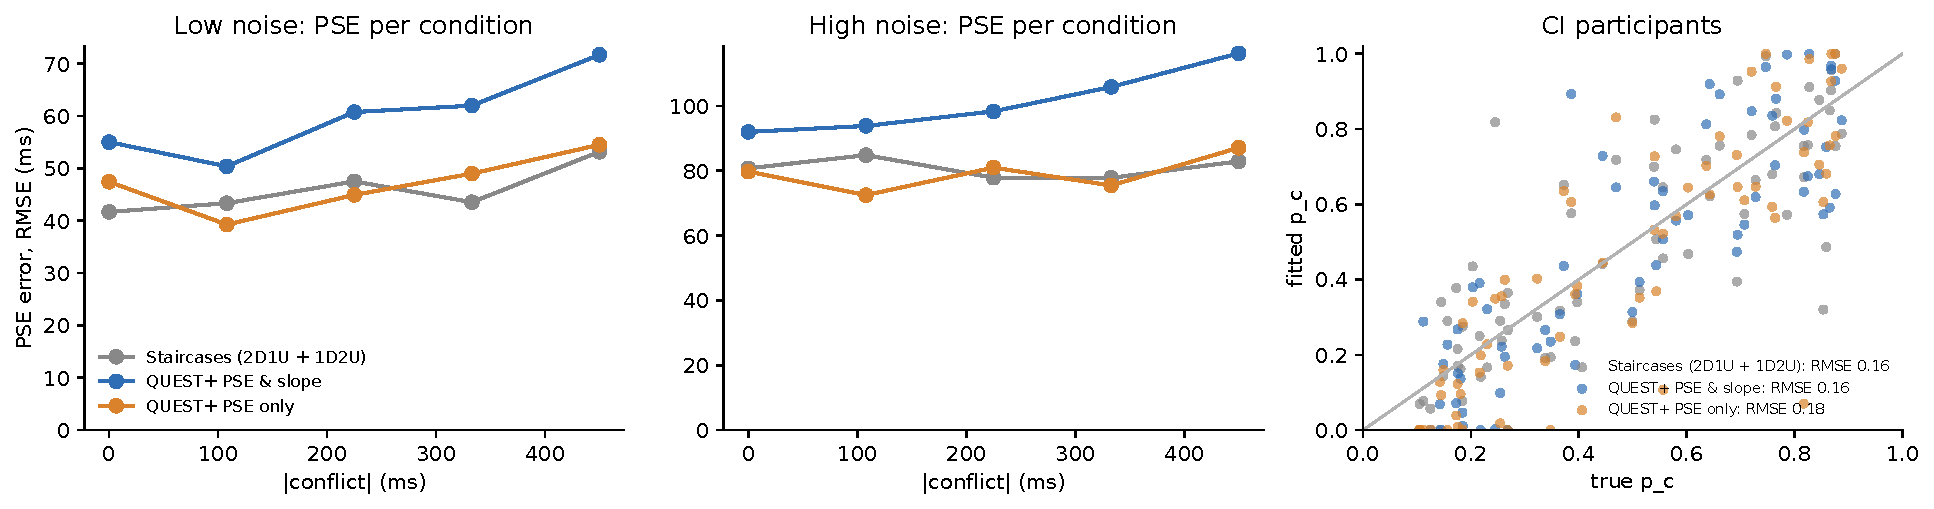
\includegraphics[width=\linewidth]{fig_qplus_pse_pc.pdf}
\caption{Main experiment, 9 conflicts $\times$ 72 trials, the same participants under each method. Top: model recovery (AIC). Bottom: PSE error per condition by $|$conflict$|$, and fitted vs true $p_c$ for CI participants.}
\label{fig:qplus}
\end{figure}

\paragraph{Why QUEST+ does not help here.}
\begin{itemize}
\item \textbf{The staircases already sample where the information is.} 2D1U and 1D2U settle near 71\% and 29\% ``test longer'', on the two flanks of the psychometric function. That is close to where trials are most informative about both the PSE and the slope. In the unimodal blocks QUEST+ was compared with a different set of staircases, the old 4-staircase design.
\item \textbf{QUEST+ optimises the wrong target.} It refines each condition's own lognormal PSE and slope. The model comparison rests on how the PSE and the slope change across conflicts, and under CI and switching the psychometric functions are mixtures, not lognormal. QUEST+ targeting PSE and slope spends trials far out on the flanks to pin down the slope, which costs PSE precision (61 vs 47\,ms) and does not buy better model recovery.
\item \textbf{The broad prior costs early trials.} Each condition has only 64 adaptive trials, and some of them go into locating a PSE that could lie anywhere from 40 to 1400\,ms. A prior centred on the fusion prediction would reduce this, but probably not enough to change the conclusion.
\end{itemize}
Under BIC, QUEST+ recovers switching participants more often (63--69\% vs 53\%), because it samples the flanks where the two switching slopes differ. Under AIC, which this report recommends, the staircases are as good or better.

A model-based design would be needed for real gains: choosing the conflict and test duration that best separate CI, fusion and switching, given the data so far. That is a much larger change and was not simulated.

\paragraph{The main design itself.} The staircase numbers here also confirm the main-experiment recommendation, with $\sigma_V$ as precise as a joint fit provides. At 72 trials per condition: model recovery 90\% (AIC), CI recognised in 90\% of cases, and $p_c$ RMSE 0.16 ($r = 0.83$). That is at least as good as 154 trials per condition with $\sigma_V$ free (80\%, $p_c$ RMSE 0.29).

\section{Bigger picture: making the experiment shorter and more reasonable}\label{sec:ideas}
\begin{enumerate}
\item \textbf{Model the bias instead of correcting it.} Fit $\ln\hat s_V = \ln s_V - c - d\ln(s_V/0.5)$ inside the CI fit: $c$ per participant and noise level from the cross-modal block, $d$ shared (or per participant once everyone has 3 standards). The main experiment then needs no per-participant bias correction, and no pause to compute it between the cross-modal and main blocks. The simulations above assume exactly this.
\item \textbf{Cross-modal standards that cover the main experiment.} With 9 conflicts the visual standards run from 50 to 950\,ms, but the bias is measured at 300--800\,ms. Standards of, for example, 150/500/900\,ms would turn the extrapolation into an interpolation. The shared log-linear model handles a change of standards for new participants without trouble.
\item \textbf{$\sigma_V$ (and possibly $\sigma_A$) from the unimodal blocks.} This was the single biggest gain in the simulations (Section~\ref{sec:bimodal}), and it makes the unimodal blocks part of the model rather than a screening step. Of the possible improvements, it most deserves the extra visual trials.
\item \textbf{Fewer easy trials.} The fits share one lapse rate across conditions, so 14 easy trials in every main-experiment condition (196 trials, 10\,min) are more than the lapse estimate needs. The proposed 8 per condition (144 trials) still screens each condition and anchors each condition's psychometric curve. I would not go lower.
\item \textbf{Split the main experiment into resumable parts.} At 67\,min it can run as two 35-minute parts (all conditions interleaved in each), on the same day or on two days. The bias model makes the order of parts unimportant.
\item \textbf{Noise calibration.} It did not predict the unimodal $\sigma$ at the calibrated level: P101 0.74 predicted vs 0.42 measured, P103 0.68 vs 2.68, P104 0.72 vs 0.47. Two options:
  \begin{itemize}
  \item shorten it to 60 trials per staircase (about 6\,min, as before);
  \item drop it and use a fixed high-noise level, checked by the unimodal auditory block, which measures $\sigma$ at that level anyway.
  \end{itemize}
  Either option saves 4--11\,min. The second needs a look at the spread of $\sigma$ at a fixed level in v1 (2 of 11 participants were at chance at 1.2).
\item \textbf{QUEST+ in the main experiment: no} (Section~\ref{sec:qplus}). Per-condition QUEST+ did not beat the staircases. A model-based design (choosing the conflict and test duration that best discriminate the models) is possible in principle, but it is complex and fragile in a running experiment. With the joint fit already reaching 90\% model recovery, it is not worth it now.
\end{enumerate}

\section{Limitations}
\begin{itemize}
\item No audiovisual bias was simulated in the main experiment. An error in the bias model would show up as a shifted PSE-vs-conflict curve, which CI and fusion explain differently.
\item Fixing $\sigma_V$ assumes the unimodal and bimodal visual noise are the same.
\item Parameters were drawn from broad uniform ranges, and real participants may cluster elsewhere (for example $p_c$ near 1).
\item With 46--55 simulated participants per model, recovery rates carry an error of about $\pm$6 points. Differences smaller than about 10 points (for example weighted vs equal allocation) are not reliable.
\item The trials-to-minutes conversion (3.1\,s) is measured, but breaks and instructions between blocks are not included.
\end{itemize}

\paragraph{Files.} \texttt{analysis/overnight\_sims/}: \texttt{avmodels.py} (quadrature likelihood), \texttt{adaptive\_sims.py}, \texttt{bimodal\_recovery.py}, \texttt{fixed\_sv.py}, \texttt{qplus\_main.py}, \texttt{analyse.py}; raw results in \texttt{results/}, tables (\texttt{*.csv}) and figures in \texttt{report/}.

\appendix
\section{Further figures}
\begin{figure}[h]
\centering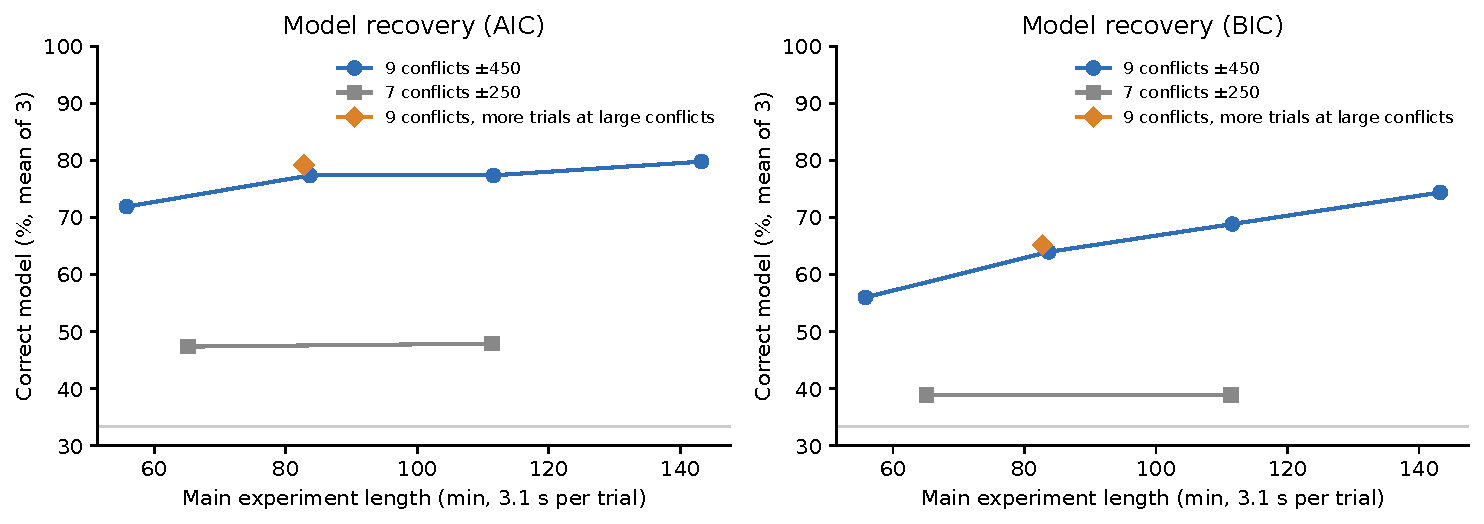
\includegraphics[width=0.9\linewidth]{fig_recovery_vs_time.pdf}
\caption{Mean correct model recovery against the main experiment's length ($\sigma_V$ fitted).}
\label{fig:time}
\end{figure}
\begin{figure}[h]
\centering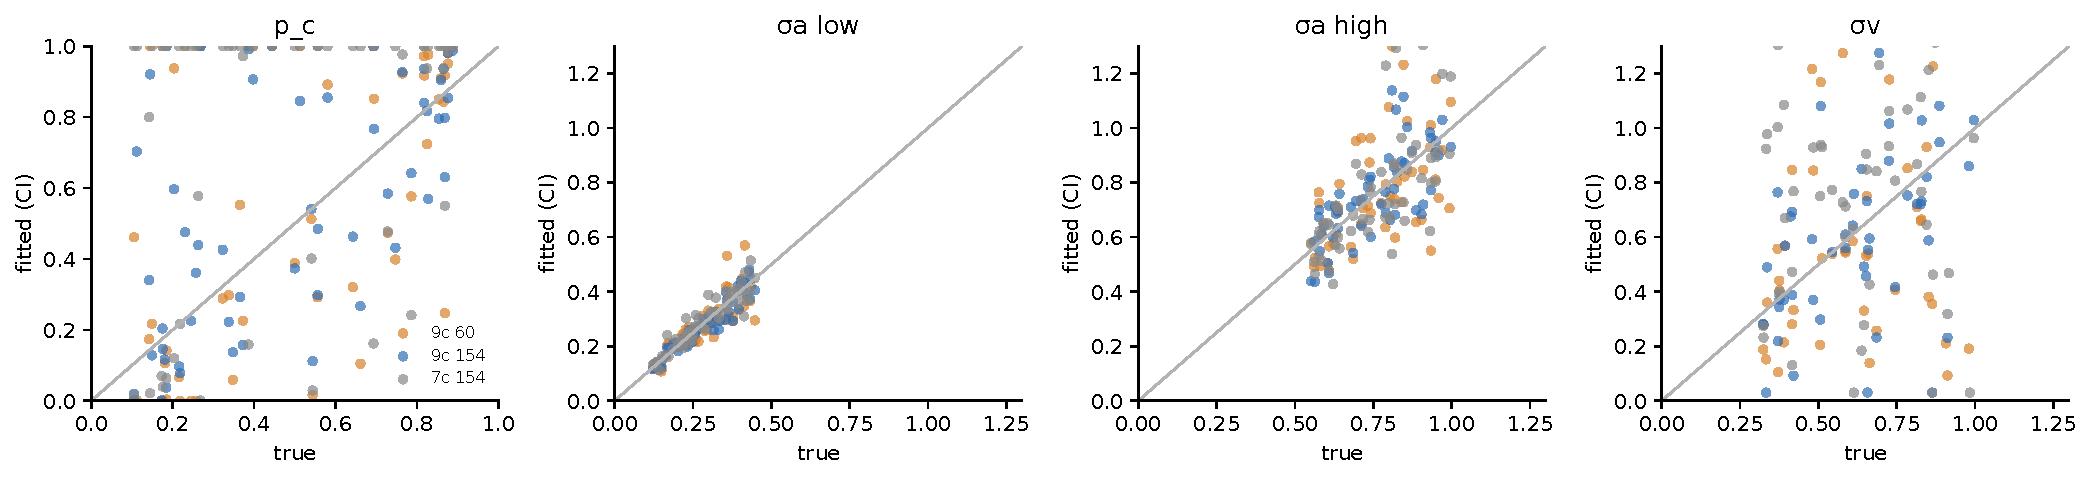
\includegraphics[width=\linewidth]{fig_ci_params.pdf}
\caption{CI parameters for CI participants, $\sigma_V$ fitted (9 conflicts at 60 and 154 trials, 7 conflicts at 154).}
\label{fig:ci}
\end{figure}
\begin{figure}[h]
\centering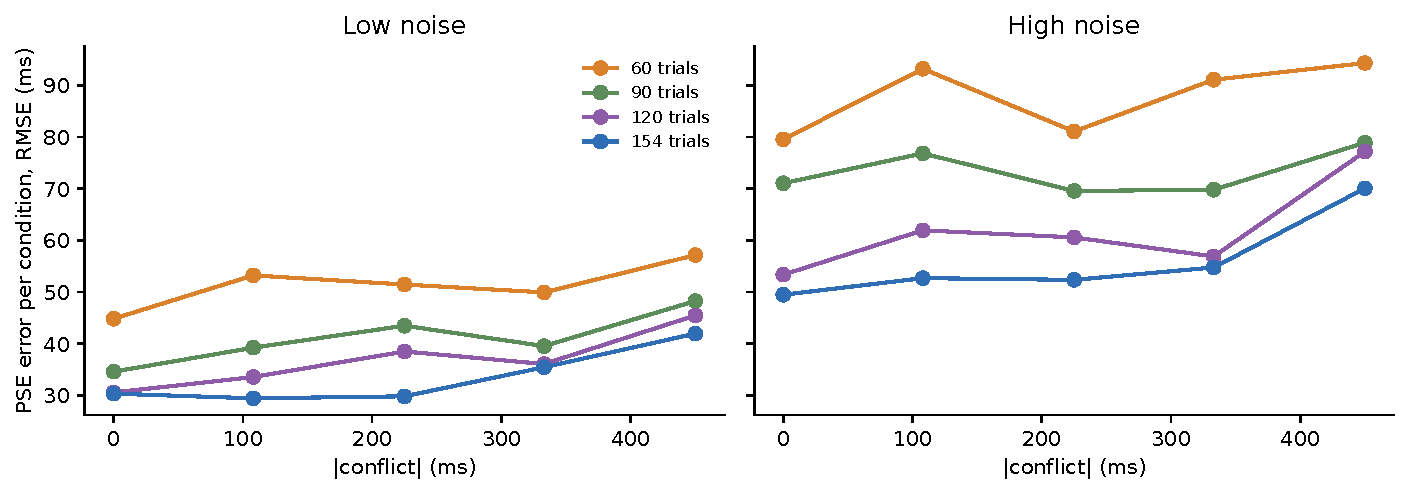
\includegraphics[width=0.85\linewidth]{fig_pse_precision.pdf}
\caption{PSE error per condition (lognormal fit per condition) against $|$conflict$|$, 9 conflicts.}
\label{fig:pse}
\end{figure}
\end{document}
